\documentclass{article}

\usepackage{polski}
\usepackage{amsmath, array}
\usepackage{graphicx}
\usepackage{float}
\usepackage{subfig}
\usepackage{multirow}
\usepackage{enumitem}

\title{Laboratorium 12}
\author{\textbf{Łukasz Wala}\\
    \textit{AGH, Wydział Informatyki, Elektroniki i Telekomunikacji} \\
    \textit{Teoria Współbieżności 2022/23}}
\date{Kraków, \today}

\begin{document}
\maketitle

\section{Zadania}

\subsection{Zadanie 1}
Wymyślić własną maszynę stanów, zasymulować przykład i dokonać analizy grafu osiągalności oraz niezmienników.

\begin{figure}[H]
    \centering
    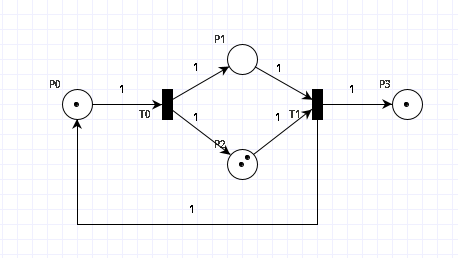
\includegraphics[width=\textwidth]{net_1.png}
    \caption{Maszyna stanów}
\end{figure}

\begin{figure}[H]
    \centering
    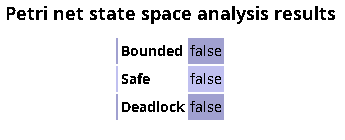
\includegraphics[width=0.7\textwidth]{analysis_1.png}
    \caption{Wynik dla \textit{State Space Analysis}}
\end{figure}

Sieć nie jest ograniczona, ponieważ w P3 będzie przybywać tokenów w nieskończoność, z tej racji nie jest 
również bezpieczna (1-ograniczona). Nie ma deadlock-a, ponieważ zawsze jest możliwość wykonania każdego z
przejść.

\begin{figure}[H]
    \centering
    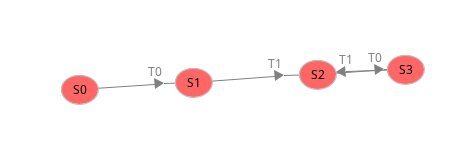
\includegraphics[width=0.7\textwidth]{reachability_1.png}
    \caption{Wykres \textit{Reachablility/Coverability Graph}}
\end{figure}

Każde ze znakowań jest osiągalne, każde z przejść jest żywe, czyli sieć również jest żywa.

\begin{figure}[H]
    \centering
    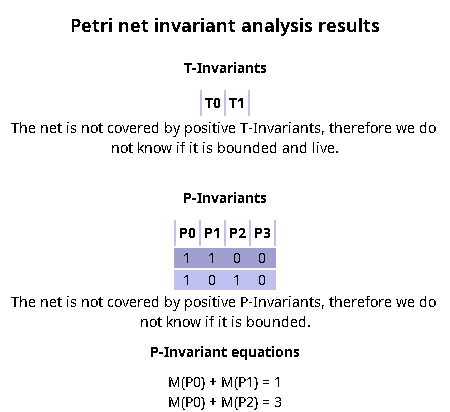
\includegraphics[width=0.7\textwidth]{invariant_1.png}
    \caption{Wynik \textit{Invariant analysis}}
\end{figure}

\textit{T-invariants} jest puste, co sugeruje, że sieć jest nieodwracalna.

\subsection{Zadanie 2}
Zasymulować sieć jak poniżej. Dokonać analizy przejść. Jaki wniosek można wyciągnąć o odwracalności
sieci? Wygenerować graf osiągalności. Proszę wywnioskować z grafu, czy sieć jest żywa.
Proszę wywnioskować czy jest ograniczona. Objaśnić wniosek.

\begin{figure}[H]
    \centering
    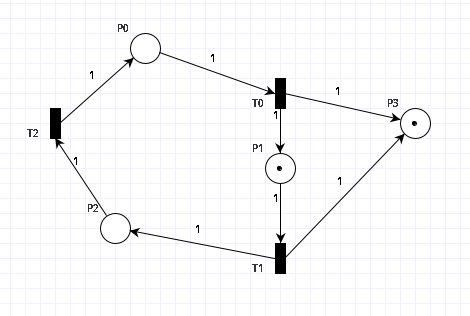
\includegraphics[width=0.7\textwidth]{net_2.png}
\end{figure}

\begin{figure}[H]
    \centering
    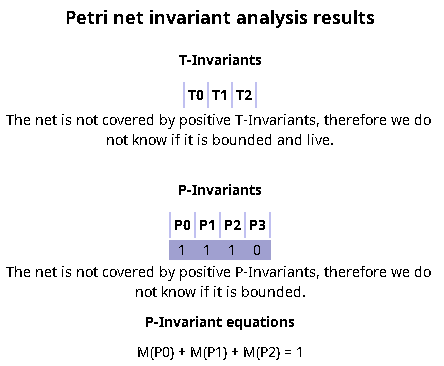
\includegraphics[width=0.7\textwidth]{invariant_2.png}
    \caption{Wynik \textit{Invariant analysis}}
\end{figure}

\begin{figure}[H]
    \centering
    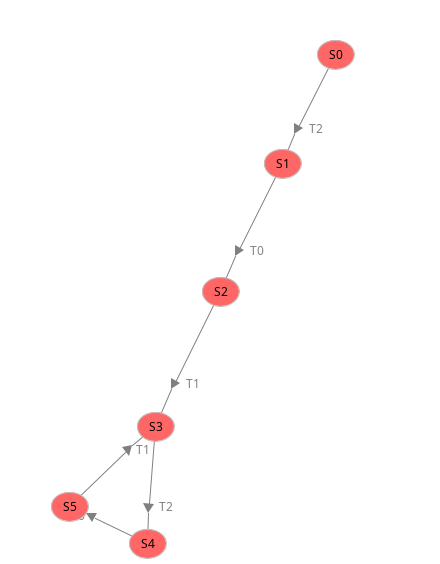
\includegraphics[width=0.7\textwidth]{graph_2.png}
    \caption{Wynik \textit{Reachability/Coverability Graph}}
\end{figure}

Brak odwracalności, co można stwierdzić na podstawie braku wektora \textit{T-invariants}.
Sieć jest żywa - każde przejście musi się wykonać, następnie wykonują się w pętli.
Nie jest ograniczona, liczba tokenów w P3 rośnie w nieskończoność.

\subsection{Zadanie 3}
Zasymulować wzajemne wykluczanie się dwóc procesów na wspólnym zasobie. Dokonać analizy niezmienników.
Wyjaśnić znaczenie równań (\textit{P-invariant equations}). Czy sieś jest zachowawcza? Które równanie
mówi nam o rozmiarze bufora?

\begin{figure}[H]
    \centering
    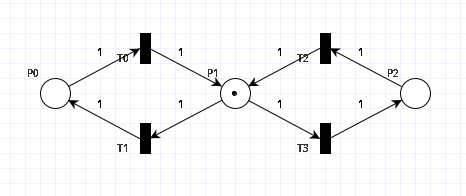
\includegraphics[width=0.7\textwidth]{net_3.png}
    \caption{Sieć przedstawiająca wykluczające się procesy}
\end{figure}

Znakowanie P1 oznacza stan wolny zasobu, znakowania P0 oraz P1 "konkurują" o zasób.

\begin{figure}[H]
    \centering
    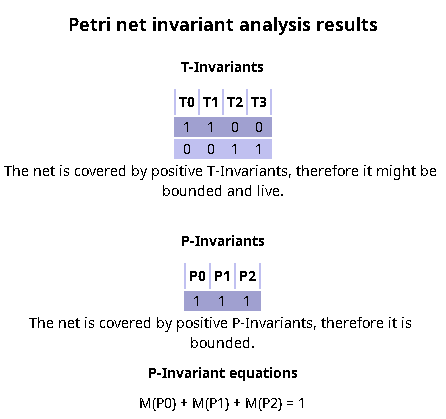
\includegraphics[width=0.7\textwidth]{invariant_3.png}
    \caption{Wynik \textit{Invariant analysis}}
\end{figure}

W równaniu występują wszystkie trzy znakowania. Znakowanie P1 oznacza że zasób jest wolny, P0 oraz P2
oznaczają, że zasób jest zajęty przez jeden z procesów. Liczba jeden po prawej stronie równania
oznacza, że suma tokenów we wszystkich stanach zawsze wynosi jeden, czyli token zawszy musi 
być tylko w jednym ze znakowań, dzięki temu zasób jest chroniony przed jednoczesnym dostępem przez dwa
procesy.

\subsection{Zadanie 4}
Uruchomić problem producenta i konsumenra z ograniczonym buforem. Dokonać analizy niezmienników.
Czy sieć jest zachowawcza? Które równanie nam o rozmiarze bufora?

\begin{figure}[H]
    \centering
    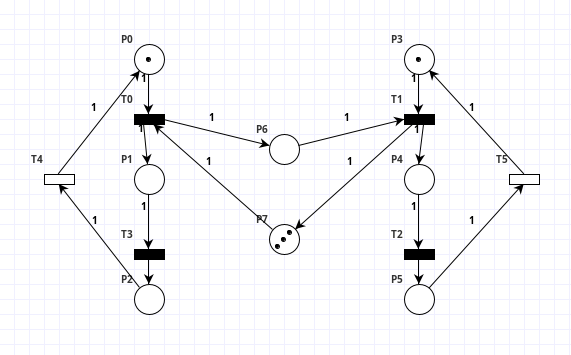
\includegraphics[width=0.7\textwidth]{net_4.png}
    \caption{Sieć dla problemu producenta i konsumenta}
\end{figure}

\begin{figure}[H]
    \centering
    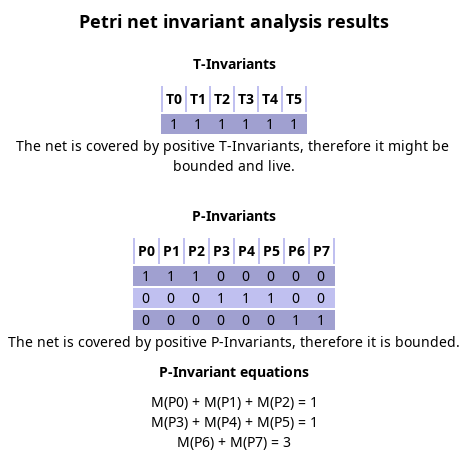
\includegraphics[width=0.7\textwidth]{invariant_4.png}
    \caption{Wynik \textit{Invariant analysis}}
\end{figure}

Sieć jest zachowawcza, ponieważ każde przejście produkuje tyle samo tokenów ile pobiera.
Na podstawie \textit{T-Invariants} można wnioskować, że sieć jest odwracalna. Sieć jest
żywa, ponieważ wszystkie przejścia mogą być wykonane. O wielkości bufora mówi równanie
trzecie, znakowanie P6 odpowiada za miejsca zajęte, a P7 za miejsca wolne.

\subsection{Zadanie 5}
Stworzyć symulację problemu producenta i konsumenta z nieograniczonym buforem. Dokonać analizy niezmienników.
Zaobserwować brak pełnego pokrycia miejsc.

\begin{figure}[H]
    \centering
    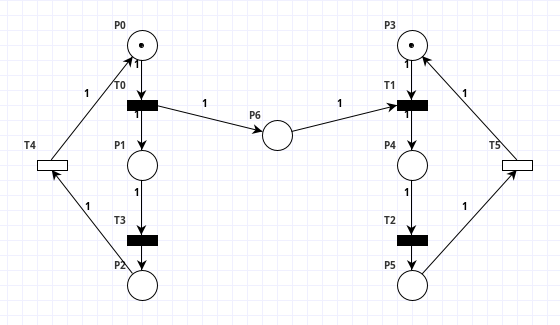
\includegraphics[width=0.7\textwidth]{net_5.png}
    \caption{Sieć dla problemu producenta i konsumenta z nieograniczonym buforem}
\end{figure}

\begin{figure}[H]
    \centering
    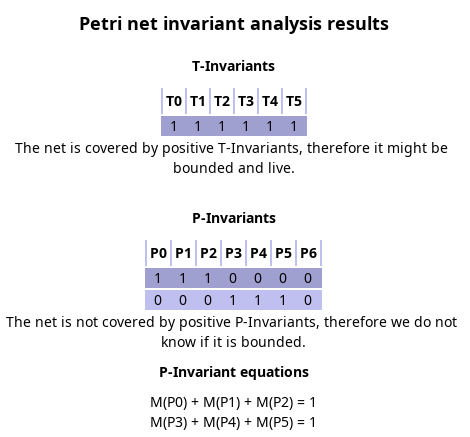
\includegraphics[width=0.7\textwidth]{invariant_5.png}
    \caption{Wynik \textit{Invariant analysis}}
\end{figure}

Na podstawie wektora \textit{T-invariants} widać, że sieć jest odwracalna.
Jest też żywa, ponieważ każde znakowanie jest osiągalne.
Brak równania zawierającego P6 w sekcji \textit{P=invariants} oznacza, że to znakowanie
(symbolizujące bufor) jest nieograniczone.

\subsection{Zadanie 6}
Zasymulować prosty przykład ilustrujący zakleszczenie. Wygenerować graf osiągalności i zaobserwować
znakowania, z których nie można wykonać przejść. Zaobserwować właściwości sieci w \textit{State Space Analysis}.
Poniżej przykład sieci z możliwością zakleszczenia.

\begin{figure}[H]
    \centering
    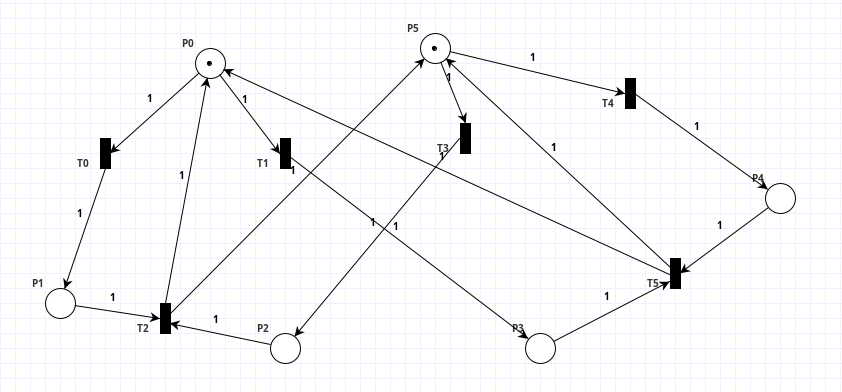
\includegraphics[width=0.7\textwidth]{net_6.png}
    \caption{Przykład sieci z zakleszczeniem}
\end{figure}

\begin{figure}[H]
    \centering
    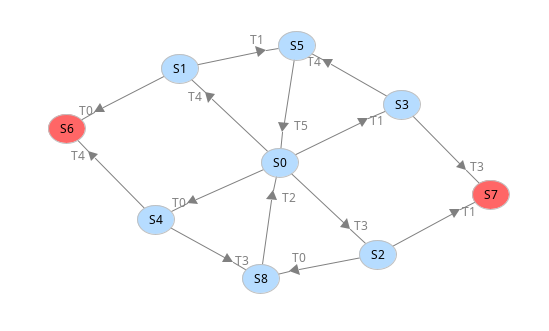
\includegraphics[width=0.7\textwidth]{graph_6.png}
    \caption{Wynik \textit{Reachability/Coverability Graph}}
\end{figure}

Graf łatwo pozwala stwierdzić, że stanami, w których nastąpi deadlock, są S6 oraz S7.

\begin{figure}[H]
    \centering
    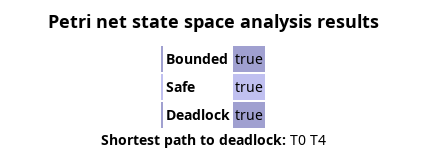
\includegraphics[width=0.7\textwidth]{analysis_6.png}
    \caption{Wynik \textit{State Space Analysis}}
\end{figure}

Powyżej wydać, że najkrótszą ścieżką do zakleszczenia są przejścia T0 oraz T4.

\section{Wnioski}
Powyższe przykłady pokazują możliwości sieci Petriego do formalnego modelowania problemów
współbieżnych, np. problemu producentów i konsumentów. Dzięki takiemu formalnemu modelowi
można zbadać pewne właściwości problemu, jego przebieg, co może być przydatne przy np.
unikaniu zakleszczeń czy innych rodzajów niepowodzeń.

\section{Bibliografia}

\begin{enumerate}
    \item
    N.J. Dingle, W.J. Knottenbelt and T. Suto. PIPE2: A Tool for the Performance Evaluation of Generalised Stochastic Petri Nets
\end{enumerate}

\end{document}